\section{Трекинг на основе особых точек и цвета}\label{tracking}

Данный раздел содержит описание предлагаемого алгоритма трекинга,
комбинирующего в себе два подхода: основанный на ключевых точках
и основанный на цветах.
Сначала идет описание части метода, использующей точечные особенности
изображения.
Оно является достаточно кратким, поскольку рассказывает о довольно
распространенном и известном подходе.
Затем идет описание части, использующей цветовую информацию.
Оно является более подробным, поскольку касается менее распространённого
подхода и содержит некоторые модификации.
Завершается раздел описанием способа комбинирования цветового и точечного
алгоритмов.

\subsection{Трекинг на основе точечных особенностей изображения}
\label{subs:feat_tracking}

Применяемый в данной работе алгоритм трекинга с помощью точечных особенностей
представляет собой разновидность стандартного подхода "--- трекера
Канаде "--- Лукаса "--- Томаси
(KLT-трекера)\cite{LucasAndKanade,TomasiAndKanade,ShiAndTomasi,PyrLK}.
На кадрах с известной позицией объекта выделяются ключевые 2D-точки (точечные
особенности) и определяются соответствующие им 3D-точки на поверхности модели.
Движение ключевых точек от кадра к кадру отслеживается с помощью вычисления
оптического потока.
На кадре, для которого выполняется оценка позиции, по известным 2D-3D
соответствиям вычисляется положение объекта путем решения задачи
\PnP\cite{LepetitSurvey} с использованием RANSAC\cite{RANSAC} для отсеивания
выбросов.

\Comment{TODO: о порядке репроецирования 3D-точек, отбрасывании треков
и пересчете 3D-позиций рассказать подробнее в разделе про комбинирование.
Возможно, здесь нужно будет кратко на это сослаться.}

\subsection{Метод на основе распределения цвета}

\Comment{Во всем разделе плохо с обозначениями и формулами.}

\newcommand{\Hf}{\ensuremath{H_f}}
\newcommand{\Hb}{\ensuremath{H_b}}
\newcommand{\uvec}{\ensuremath{\vect{u}}}
\newcommand{\xvec}{\ensuremath{\vect{x}}}
\newcommand{\hedist}{\ensuremath{\HeX{\CDistX{\uvec}}}}
\newcommand{\HistLocal}{\ensuremath{H_i}}
\newcommand{\HistLocalFg}{\ensuremath{{\Hf}_i}}
\newcommand{\HistLocalBg}{\ensuremath{{\Hb}_i}}

Метод, использующий распределение цветов, направлен на нахождение такой
позиции, при которой контур наилучшим образом отделяет передний план от фона.
Это означает, что цвета на $\FgProj$ будут соответствовать цветам,
встречавшимся на переднем плане ранее в ходе трекинга, и наоборот: точки,
оказавшиеся на $\BgProj$, будут иметь цвет, характерный для фона.

На каждом кадре после вычисления позиции объекта собираются данные по цветам
точек на переднем плане и на фоне.
Затем эти данные объединяются с общей статистикой, собранной в ходе трекинга.
Статистика собирается в окрестности контура объекта.
Эта окрестность, обозначаемая $\CtLocal$, разбивается на несколько
непересекающихся областей~$\{\CtLocal_i\}_{i = 1}^n$.
Каждая из этих областей включает в себя часть переднего плана и часть фона:

\begin{align}
\label{eqn:histo_partitioning}
\CtLocal_i &= {\CtLocalFg}_i \cup {\CtLocalBg}_i \\
{\CtLocalFg}_i &= \CtLocal_i \cap \CtLocalFg \\
{\CtLocalBg}_i &= \CtLocal_i \cap \CtLocalBg
\text{.}
\end{align}

Подробнее о том, как окрестность контура разбивается на локальные области,
будет
рассказано в следующем разделе.

Цветовая статистика ведётся для каждой из областей ${\CtLocalFg}_i,
{\CtLocalBg}_i$ отдельно, для того чтобы отдельно учитывать цветовые
особенности разных сторон объекта.
Для её хранения и обновления используются гистограммы распределения цветов.
Перед построением гистограмм изображение преобразуется так, чтобы цвет в каждом
канале принимал значение от $0$ до $31$.
Таким образом, каждая гистограмма состоит из $32^3$ ячеек.
В каждую ячейку гистограммы ${\HistLocal}_j$ записывается доля пикселей
соответствующего цвета на её области ${\CtLocal_i}_j$.

Для данного цвета $y$ значения в гистограммах $\HistLocalFg(y)$ и
$\HistLocalBg(y)$ "--- это вероятности точки иметь цвет $y$, находясь
соответственно на переднем плане или на фоне.
Из-за того, что для в каждой локальной области существует своя пара гистограмм,
эти вероятности могут быть разными на разных участках изображения.

\begin{align}
\label{eqn:H_f_Y}
    \HistLocalFg(y) &= \probX{I(\uvec) = y \mid \uvec \in \FgProj} \\
    \HistLocalBg(y) &= \probX{I(\uvec) = y \mid \uvec \in \BgProj}
\text{.}
\end{align}

На новом кадре собранная статистика позволяет для каждой возможной позиции
объекта оценить её апостериорную вероятность при данном изображении и данном
наборе гистограмм.
Пусть дан новый кадр и некоторая позиция $\Pose$.
Спроецируем объект на изображение с использованием этой позиции.
Получим контур $\Contour$ и разбиение его окрестности на локальные области.
Тогда, как и в~\cite{Hexner2016}, вероятность того, что $\Pose$ является
позицией объекта, можем оценить как

\begin{equation}
\label{eqn:pos_prob}
    \probMainX{\Pose} = \prod\limits_{\uvec \in \CtLocal} \left(
        \probF{\uvec} \hedist
        + \probB{\uvec} \left( 1 - \hedist \right)
    \right)
\text{.}
\end{equation}

Здесь $\He$ "--- приближение функции Хевисайда:

\begin{equation}
\label{eqn:heaviside}
    \HeX{x} = \frac{1}{\pi} \left( \arctan(\alpha x) - \frac{\pi}{2} \right)
\text{.}
\end{equation}

$\probF{\uvec}$ и $\probB{\uvec}$ "--- вероятности попадания точки $\uvec$ на
передний план и на фон в соответствии с её цветом:

\begin{align}
\label{eqn:Pfu}
    \probF{\uvec} &= \frac{\HistLocalFg(y)\eta_f}{\HistLocalFg(y)\eta_f +
        \HistLocalBg(y)\eta_b} \text{,} \\
    \probB{\uvec} &=\frac{\HistLocalBg(y)\eta_b}{\HistLocalFg(y)\eta_f +
        \HistLocalBg(y)\eta_b} \text{,}
\end{align}

где
$
    \eta_f = \sum\limits_{\uvec \in \CtLocal_i}\hedist
$ "--- количество точек переднего плана на $\CtLocal_i$,

$
    \eta_b = \sum\limits_{\uvec \in \CtLocal_i}(1 - \hedist)
$ "--- количество точек фона.

$\He$ оценивает вероятность того, что $\uvec$ лежит на переднем плане, с точки
зрения позиции объекта, а $\probF{\uvec}$ "--- с точки зрения цвета.

Таким образом, вероятность позиции $\Pose$ будет высокой, если точки области
$\CtLocalFg$ будут по цвету классифицироваться как точки переднего плана, а
точки области $\CtLocalBg$ "--- как фон.

Процесс вычисления позиции на новом кадре состоит в максимизации вероятности
$\probMainX{\Pose}$ или, что то же самое, в минимизации функции энергии
цветового трекинга.
Эта энергия получается логарифмированием и умножением на $-1$
формулы~\ref{eqn:pos_prob}:

\begin{equation}
\label{eqn:err_func}
\Energy(\xi) = - \sum\limits_{\uvec \in \CtLocal}
\log(\hedist \probF{\uvec} + (1 - \hedist)\probB{\uvec})
\text{.}
\end{equation}

Оптимизация проводится квазиньютоновским методом последовательного
квадратичного программирования (SLSQP)~\cite{SLSQP}.
Градиент вычисляется аналитически.
Вывод формулы градиента можно найти в~\cite{Tjaden2018}.
\Comment{Подсчет градиента на самом деле отличается от \cite{Tjaden2018}}

Позиция объекта при оптимизации параметризуется шестью параметрами:
задающими вращение объекта относительно начального положения углами Эйлера
и трехмерным вектором параллельного переноса.
Перед началом трекинга размер 3D-модели меняется так, чтобы её диаметр равнялся
$5$.
Делается это для того, чтобы уровнять влияние отвечающих за вращение и
параллельный перенос параметров.

Метод SLSQP позволяет задавать ограничения на область оптимизации.
Для параметров переноса мы ограничиваем ширину области величиной $kd$,
где $d$ "--- диаметр объекта.
Ширина области для параметров поворота "--- $m$ радиан (в нашей реализации $d
=0.4, m = 1$).
Центром области является начальная позиция объекта.
Благодаря ограничениям результат оптимизации не будет слишком далёк от точки
инициализации даже при неблагоприятных для трекинга условиях и зашумлённой
функции энергии.
Также эти ограничения позволяют избежать складывания рамок, которое
могло бы возникнуть из-за использования углов Эйлера.

После получения новой позиции на каждом следующем кадре строятся новые
гистограммы, которые взвешенно суммируются со старыми:

\begin{align}
\HistLocalFg &= \alpha_f \HistLocalFg^{\text{\it new}} + (1 - \alpha_f)
\HistLocalFg^{\text{\it old}} \\\HistLocalBg &= \alpha_b
\HistLocalBg^{\text{\it new}} + (1 - \alpha_b) \HistLocalBg^{\text{\it
old}}\text{,}
\end{align}

где $\alpha_f, \alpha_b$ - коэффициенты обновления (в нашей реализации
$\alpha_f = 0.1, \alpha_b = 0.2$).

\subsubsection*{Разбиение на локальные области}

Оптимизация функции ошибки~\ref{eqn:err_func} направлена на нахождение такой
позиции, при которой контур лучше всего отделяет передний план от фона.
Для этого её вычисление проводится по полосе вокруг контура ширины $2r$ (в нашей
реализации $r = 40$).
Эта полоса разбивается на $32$ локальные области, для каждой из
которых поддерживается одна пара гистограмм.

Области должны, по возможности, содержать примерно равное количество точек
переднего плана и фона, то есть внутренней и внешней частей полосы.
Поэтому они строятся так, чтобы контур проходил по середине области: область
точки на полосе совпадает в предлагаемом решении с областью ближайшей
к ней точки на контуре (рис.~\ref{fig:fb_contour}).

\begin{figure}[t]
\centering
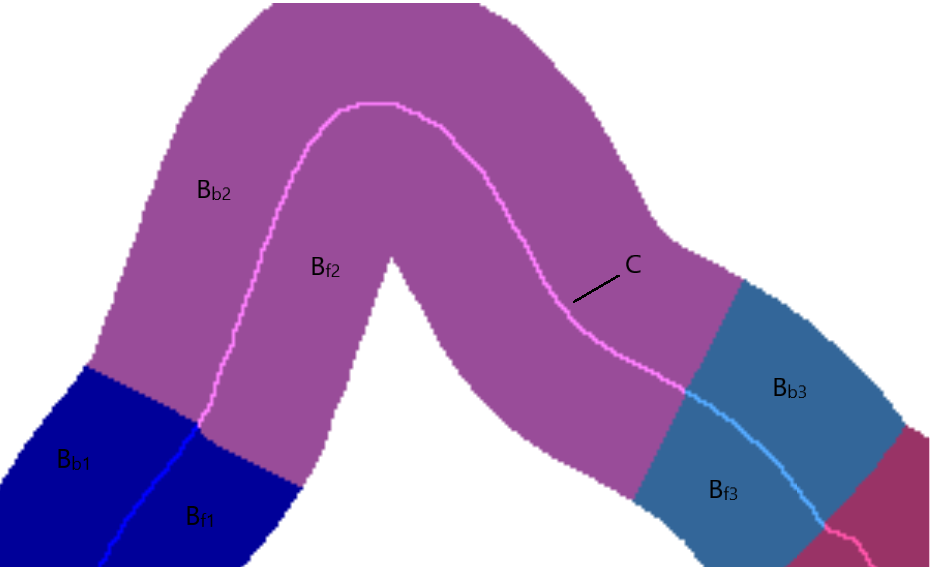
\includegraphics[width=\textwidth]{fig/fb_contour.png}
\caption{
Разбиение на области ${B_f}_i, {B_b}_i$ полосы вокруг контура, по которой
вычисляется функция ошибки
} \label{fig:fb_contour}
\end{figure}

Таким образом, для разбиения полосы достаточно разбить на области точки контура.
Для этого на участки делится поверхность трёхмерной модели
объекта: объект помещается в центр единичной сферы, а сама сфера разбивается
на $32$ равные по площади части по зенитным и азимутным углам.
Каждую точку объекта можно отнормировать, чтобы она попала на поверхность
сферы, и таким образом поделить на области поверхность объекта
(рис.~\ref{fig:color-object-areas}).
Проекция объекта позволяет поделить на области контур
(рис.~\ref{fig:projected-areas}).

\begin{figure}[t]
\centering
\begin{minipage}[h]{0.49\linewidth}
\center{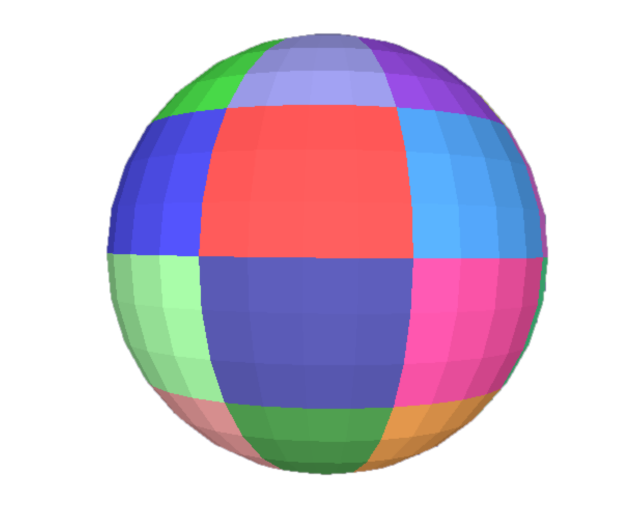
\includegraphics[width=0.8\linewidth]{fig/sphere_straight.png}}
\end{minipage}
\hfill
\begin{minipage}[h]{0.49\linewidth}
\center{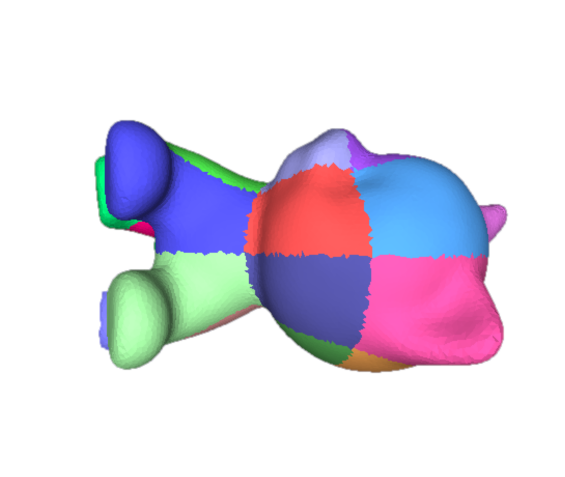
\includegraphics[width=0.8\linewidth]{fig/cat_straight.png}}
\end{minipage}
\caption{Разбиение на локальные области поверхностей сферы и объекта}
\label{fig:color-object-areas}
\end{figure}

\begin{figure}[t]
\centering
\begin{minipage}[h]{0.49\linewidth}
\center{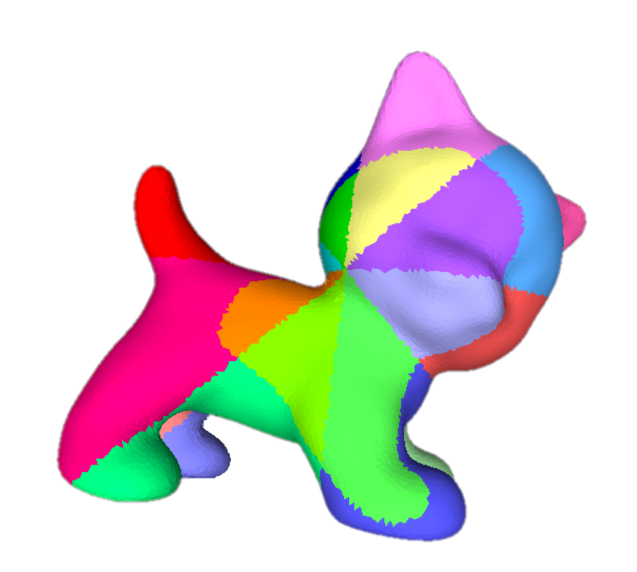
\includegraphics[width=0.8\linewidth]{fig/cat_transformed.png}}
\end{minipage}
\hfill
\begin{minipage}[h]{0.49\linewidth}
\center{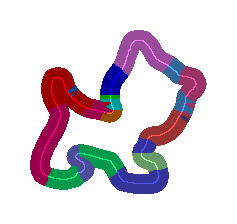
\includegraphics[width=0.8\linewidth]{fig/cat_contour.png}}
\end{minipage}
\caption{Слева разбиение на области 3D-модели объекта. Проекция объекта
разбивает на области контур (правое изображение). Точки вокруг контура
поппадают в ту же область, что и ближайшие точки на контуре. }
\label{fig:projected-areas}
\end{figure}

Такое разделение объекта неизменно между кадрами, поэтому цветовую информацию
в гистограммах можно накапливать в ходе трекинга.
Данные в гистограммах $\HistLocalFg$ будут при этом отражать распределение
цветов на определённых областях объекта, а данные в гистограммах
$\HistLocalBg$"--- распределение цветов на фоне вокруг этих областей.
Количество гистограмм не зависит от размера 3D-модели и остаётся небольшим, что
положительно влияет на время работы метода и позволяет обновлять все гистограммы
на каждом кадре.

На локальные области разделяется весь объект целиком.
При этом очевидно, что на отдельном кадре только часть областей будут
спроецированы на контур и поучаствуют в разбиении изображения.
Поэтому информация в некоторых гистограммах может не набираться на протяжении
большого количества кадров.
После поворота объекта такие области могут понадобиться, но информации в
их гистограммах будет недостаточно.
Для решения этой проблемы ведётся учёт <<опыта>> локальных гистограмм и
заводится одна глобальная гистограмма.

Если опыт $s_{\text{\it local}}$ пары гистограмм $\left( \HistLocalFg,
\HistLocalBg \right)$меньше некоторого порога
$s_{\text{\it suff}}$, то для точек области $\ImgDom_i$ $\Hf(y)$ и $\Hb(y)$
вычисляются как взвешенные суммы локальных и глобальных гистограмм:

\begin{align}
\label{eqn:histo_skill}
\Hf(y) &= \dfrac{s_{\text{\it local}} \HistLocalFg + (s_{\text{\it suff}} -
s_{\text{\it local}})
        {H_{\text {\it global}}}_f}{s_{\text{\it suff}}} \\
\Hb(y) &= \dfrac{s_{\text{\it local}} \HistLocalBg + (s_{\text{\it suff}} -
s_{\text{\it local}})
        {H_{\text {\it global}}}_b}{s_{\text{\it suff}}}
\text{.}
\end{align}

Порог $s_{\text{\it suff}}$ выбирается как среднее значение опыта по всем
локальным гистограммам.
Опыт локальной гистограммы оценивается как общее количество пикселей, попавших
когда-либо в её область.
Чтобы полученный на старых кадрах опыт учитывался с меньшим весом, чем на
новых, на каждом кадре он домножается на меньший единицы коэффициент:

\begin{equation}
s_{\text{\it local}} = \alpha_f s_{\text{\it local}}^{\text{\it new}} + (1 -
\alpha_f) s_{\text{\it local}}^{\text{\it old}}
\text{.}
\end{equation}

\Comment{TODO: описать то, как выбираются гистограммы.}

\subsection{Комбинирование методов}

\Comment{В чем суть комбинирования, просто поиск исходной позиции ключевыми
точками? Не только: еще и правильное согласование новой позиции и ключевых
точек. Оно заключает в себе: (1) репроецирование новых точек уже из новой
позиции, пересчет старых точек и отбрасывание точек с невидимых граней можно
тоже сюда же записать.}

Основная идея комбинирования алгоритмов заключается в последовательном их
применении и инициализации одного метода другим.
Ошибки цветового алгоритма часто бывают вызваны тем, что оптимизация функции
энергии сходится к локальному оптимуму.
Этого можно избежать, если точка инициализации достаточно близка к глобальному
минимуму.
Хорошая инициализация, кроме того, позволяет сократить время оптимизации
цветовой функции ошибки и повысить общую производительность метода.
Роль такой инициализации в предлагаемом методе играет результат алгоритма
ключевых точек.

\newcommand{\FeatAlg}{\ensuremath{F_{\text{\it feat}}}}
\newcommand{\ColorAlg}{\ensuremath{F_{\text {\it color}}}}
\newcommand{\PoseOnFrame}[1]{\ensuremath{\Pose^{\left( #1 \right)}}}
\newcommand{\PoseI}{\ensuremath{\PoseOnFrame{i}}}
\newcommand{\FeatPoseI}{\ensuremath{\PoseI_{\text {\it feat}}}}
\newcommand{\FeatPose}{\ensuremath{\Pose_{\text {\it feat}}}}

\newcommand{\XOld}{\ensuremath{\xvec_{\text {\it old}}}}
\newcommand{\XNew}{\ensuremath{\xvec_{\text{\it new}}}}
\newcommand{\ReprErr}[1]{\ensuremath{\vect{e}( #1 )}}

Схема комбинирования алгоритмов показана на рис.~\ref{fig:combining_schema}.

\begin{figure}[t]
\centering
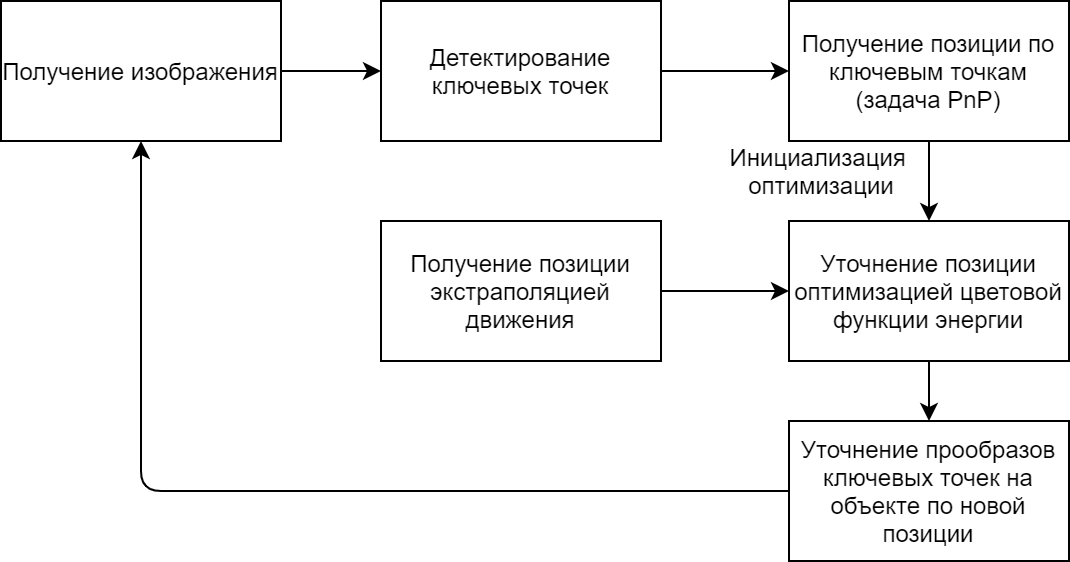
\includegraphics[width=\textwidth]{fig/combining_schema.png}
\caption{
Схема комбинирования алгоритмов
} \label{fig:combining_schema}
\end{figure}

На каждом новом кадре позиция объекта сначала вычисляется с помощью
описанного в разделе~\ref{subs:feat_tracking} метода ключевых точек.
При благоприятных условиях данная позиция будет близка к глобальному минимуму.
Если же метод ключевых точек отработал плохо (например, из-за смазанности
изображения), то эта позиция может оказаться далеко от оптимума и цветовой
алгоритм может не сойтись.
В таких ситуациях может помочь альтернативный способ инициализации,
который экстраполирует вычисленное по двум предыдущим кадрам движение объекта.
Из двух возможных начальных позиций для инициализации предлагается выбирать ту,
в которой цветовая функция ошибки покажет меньшее значение.

Полученная оптимизацией цветовой функции позиция считается уточнённой по
сравнению с полученной с помощью ключевых точек.
Поэтому эта позиция может быть использована для коррекции ключевых
точек: добавления новых 2D-3D-соответствий, уточнения и фильтрации старых.
По ней строятся обнаруженных впервые 3D-прообразы ключевых точек, при этом для
каждой точки запоминается полигон 3D-модели, на котором лежит 3D-прообраз.
Для наблюдавшихся на предыдущих кадрах точек 3D-координаты также
пересчитываются заново с использованием новой позиции объекта.
Они используются в дальнейшем вместо старых, если оказываются более точными.
Точность 3D-позиции точки определяется её ошибкой репроекции на всех кадрах,
где отслеживалась соответствующая ключевая точка.
Пусть $\XOld$ "--- старая 3D-позиция, а $\XNew$ "--- новая.
Пусть также ключевая точка была сдетектирована на изображениях начиная с
$\Img_k$
до текущего кадра $\Img_l$, и её 2D-позициями на этих кадрах были
$\uvec_k, \ldots, \uvec_l$ соответственно.
Тогда суммарной ошибкой репроекции 3D-точки $\xvec$ будет

\begin{equation}
\label{eqn:sum_reproj}
\ReprErr{\vect{x}} = \sum\limits_{i = k}^l \| \uvec_i - \projAt{\Pose_i}(\xvec) \|
\end{equation}

Старая позиция заменяется на новую, если $\ReprErr{\XNew} < \ReprErr{\XOld}$.
Так цветовой трекинг позволяет уточнить 3D-прообразы ключевых точек, тем самым
делая трекинг на ключевых точках более устойчивым.

Кроме того, с помощью уточнённой позиции проводится фильтрация выбросов:
исключаются из рассмотрения те 2D-3D-соответствия, для которых ошибка
репроекции из уточнённой позиции больше определённого порога.
Также удаляются точки, которые не попадают на передний план, то есть не лежат
на проекции объекта.
Если некоторый полигон не виден на переднем плане, то лежащие на нём точки
считаются невидимыми и тоже далее не рассматриваются.
Таким образом, уточнение позиции цветовым трекингом позволяет отфильтровать
часть 2D-3D соответствий, не согласующихся с позицией.

\Comment{Дальше идёт описание старого метода обновления 3D-позиций. В итоге
будет оставлен один из них}

Чтобы определить, какая позиция лучше, нужно оценить ошибку репроекции для
каждой позиции.
Но ошибка репроекции будет нулевой для кадра, по которому позиция вычислена,
поэтому нужно выбрать какой-то кадр, на котором обе ошибки будут отличны от
нуля.
Вопрос об обновлении позиции откладывается до следующего кадра, и решается уже
по репроекции на нём.

Пусть $\uvec_{i + 1}$ "--- позиция точечной особенности на кадре $\Img_{i +
1}$.
Пусть $\XOld$ "--- её старая 3D-позиция, а $\XNew$ "--- новая. 

Тогда ошибкой репроекции на кадре $\Img_{i + 1}$ будет

\begin{equation}
\label{eqn:err_reproj}
\ReprErr{\xvec} = \| \uvec_{i + 1} - \projAt{\Pose_i}(\xvec) \|
\end{equation}

Старая позиция заменяется на новую, если $\ReprErr{\XNew} < \ReprErr{\XOld}$.
